\documentclass[tikz,border=10pt]{standalone}
\begin{document}
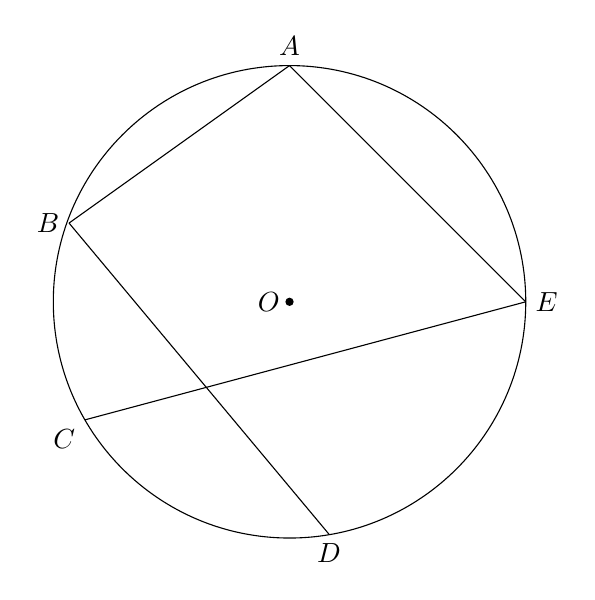
\begin{tikzpicture}
  \coordinate (O) at (0,0);
  \coordinate (A) at (0,3);
  \coordinate (B) at (-2.8,1);
  \coordinate (C) at (-2.6,-1.5);
  \coordinate (D) at (0.5,-2.95);
  \coordinate (E) at (3,0);

  \draw (O) circle (3);
  \draw (A) -- (B);
  \draw (A) -- (E);
  \draw (B) -- (D);
  \draw (C) -- (E);

  \fill (O) circle (1.5pt);

  \node[above] at (A) {$A$};
  \node[left] at (B) {$B$};
  \node[below left] at (C) {$C$};
  \node[below] at (D) {$D$};
  \node[right] at (E) {$E$};
  \node[left] at (O) {$O$};
\end{tikzpicture}
\end{document}
